203. \begin{figure}[ht!]
\center{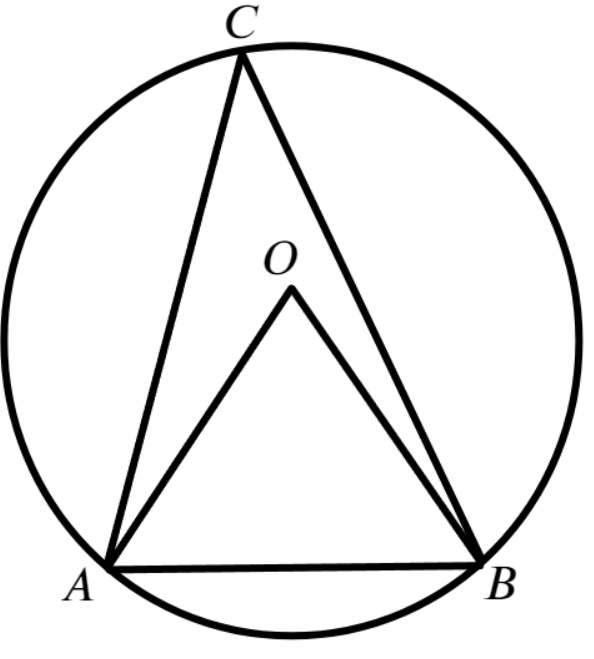
\includegraphics[scale=0.35]{g8-203.png}}
\end{figure}\\
Найдём $\angle C=180^\circ-71^\circ-79^\circ=30^\circ.$ Тогда дуга $AB$ равна $2\cdot30=60^\circ,$ а центральный угол $AOB$ также равен $60^\circ.$ В треугольнике $AOB$ стороны $AO$ и $OB$ равны радиусу, значит он равнобедренный. Так как угол при его вершине равен $60^\circ,$ он равносторонний и $AB=R=8.$\\
